
%(BEGIN_QUESTION)
% Copyright 2014, Tony R. Kuphaldt, released under the Creative Commons Attribution License (v 1.0)
% This means you may do almost anything with this work of mine, so long as you give me proper credit

Suppose a differential pressure transmitter is used to sense the level of liquid in a pressurized tank.  Both remote seals and capillary tubes on this transmitter happen to be filled with DC200 fill fluid (specific gravity = 0.934).  The process liquid is a hydrocarbon having a density of 58 pounds per cubic foot:

$$\includegraphics[width=15.5cm]{i00960x01.eps}$$

The maintenance supervisor decides to relocate the transmitter to a higher position for ease of access.  Currently it is located 6 feet above the lower remote seal, while the proposed elevation is 15 feet above the lower remote seal.  Will this shift in location necessitate {\it re-ranging} of the transmitter?  Explain why or why not.  If re-ranging is required, will the new range constitute a {\it zero shift}, a {\it span shift}, or {\it both}?

\vskip 50pt

\underbar{file i00960}
%(END_QUESTION)





%(BEGIN_ANSWER)

5 points for yes/no answer, 5 points for explanation.

\vskip 10pt

No re-ranging will be required, because although changing the transmitter's elevation will change the amount of hydrostatic pressure seen at its ports, the pressure changes will be equal at both ports and therefore will cancel each other.  In other words, it will be a {\it common-mode} pressure change and not a {\it differential} pressure change.

%(END_ANSWER)





%(BEGIN_NOTES)

{\bf This question is intended for exams only and not worksheets!}.

%(END_NOTES)

